% \subsubsection{Communication, Coordination, and Scaling}
% \label{sec:Coordination_section}

% We evaluate topology-constrained coordination using the \textsc{AGENTSNET} benchmark (Section~\ref{subsec:bench_coordination}) to isolate the coordination behavior induced by communication structures enforced in practice. Rather than ranking frameworks as software systems, we compare representative \emph{topology classes}: flexible graph-based communication (small-world, scale-free, geometric/Delaunay), role-based pipelines (sequential and hierarchical), and a centralized broadcast-like topology simulated via a fully connected graph. All benchmark settings, prompts, stopping criteria, and topology construction are fixed.\footnote{ Detailed configurations are provided in the \uline{\textcolor{blue}{\href{https://github.com/CoDS-GCS/MAFBench/blob/main/supplementary_materials/APPENDICIES.pdf}{supplementary materials}}}.}
% % All benchmark settings, prompts, stopping criteria, and topology construction are fixed, with details provided in Appendix~\ref{appendix:extended}. 
% We report success, rounds to convergence, token cost, and runtime for network sizes \(n \in \{4,8,16,50,100\}\) (Table~\ref{tab:scalability-results}). For bounded tasks, a minimum interaction budget of eight rounds is enforced. For global agreement tasks (\emph{LeaderElection} and \emph{Consensus}), we set the maximum interaction rounds to \(T = 2D + 1\), where \(D\) denotes the diameter of the communication graph\footnote{The graph diameter \(D\) is the maximum shortest-path distance between any pair of nodes in the communication graph.}, ensuring sufficient rounds for complete information propagation.


% Across all tasks, coordination outcomes are governed by the alignment between task structure and communication geometry rather than by communication volume alone. Increasing the number of rounds, tokens, or runtime does not uniformly improve success; instead, topologies succeed when they induce an information-flow pattern that matches the coordination regime, leading to pronounced success--cost trade-offs across topology classes. This effect is most evident in local coordination and negotiation tasks (\textit{Coloring} and \textit{Matching}), where graph-based topologies with local connectivity, as well as role-based hierarchical style, perform best but differ sharply in efficiency. Scale-free graphs achieve near-perfect success at scale (e.g., \(0.97\) for Coloring at \(n=100\)) while converging in fewer rounds and at substantially lower cost than small-world graphs (\(5{,}699\text{k}\) vs.\ \(10{,}431\text{k}\) tokens), reflecting hub-mediated diffusion that accelerates local agreement. Small-world graphs remain effective but incur higher coordination cost as scale increases, while geometric/Delaunay graphs exhibit substantially higher coordination burden and reduced stability, collapsing entirely for Matching at \(n=100\). Centralized broadcast (GABM-style star) topologies are excluded from Coloring as they trivially assume global neighborhood visibility, contradicting problem constraints. For Matching, they converge in very few rounds due to rapid information mixing, but achieve only moderate success at high cost, demonstrating that fast global propagation alone is insufficient to guarantee correct coordination.



% Global constraint satisfaction and agreement tasks exhibit the strongest dependence on communication topology. In \textit{VertexCover}, small-world graphs perform better at small network sizes, while scale-free graphs outperform them at large scale in both success (\(0.85\) vs.\ \(0.81\)) and cost, reflecting hub-mediated diffusion but also early decision bias at small \(n\). Leader election further exposes these limits: small-world and scale-free graphs fail across all sizes, while geometric (Delaunay) topologies succeed from moderate scale onward at high cost due to long confirmation paths. Centralized and role-based hierarchies succeed only at very small scales and degrade rapidly with size. For strict global agreement (\textit{Consensus}), the fully connected topology is strictly dominant, as it is the only structure that succeeds at all scales, converging in three rounds regardless of \(n\). All graph-based topologies fail at scale despite substantially higher coordination cost, showing that diffusion alone is insufficient for global agreement. Overall, Table~\ref{tab:scalability-results} confirms that no single topology is universally optimal, and that scalability depends on aligning task structure with communication geometry under constraints.




% Figure~\ref{fig:consensus-results} illustrates representative consensus dynamics under different topologies, highlighting fragmentation and delayed mixing in graph-based structures versus immediate convergence under broadcast. Notably, disagreement clusters persist as network size grows in sparse topologies.\footnote{Additional visualizations for all coordination tasks and topologies are provided in the \uline{\textcolor{blue}{\href{https://github.com/CoDS-GCS/MAFBench/blob/main/supplementary_materials/APPENDICIES.pdf}{supplementary materials}}}.}
 
% % Additional visualizations for all coordination tasks and topologies are provided in Appendix~\ref{appendix:extended}.



% \captionsetup[subfigure]{labelformat=empty}

\setlength{\abovecaptionskip}{2pt}
\setlength{\belowcaptionskip}{0pt}

\begin{figure*}[t]
\vspace{-2mm}
    \centering
    % --- Small sizes ---
    \subfloat[SW ($n=4$)]{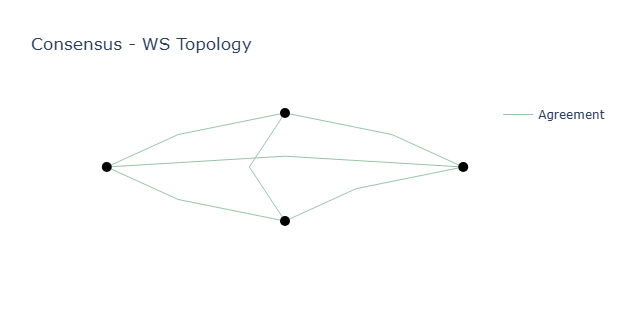
\includegraphics[trim=90 80 120 100,clip,width=0.12\textwidth]{figures/topology/consensus_results_20250917_230934_rounds3_gpt-4o-mini_nodes4.png}}
    \subfloat[SW ($n=8$)]{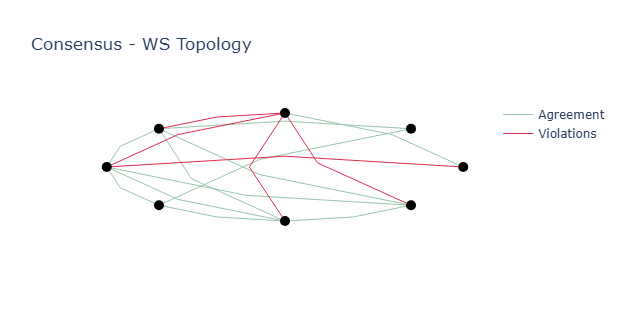
\includegraphics[trim=90 80 120 100,clip,width=0.16\textwidth]{figures/topology/consensus_results_20250917_231133_rounds7_gpt-4o-mini_nodes8.png}}
    \subfloat[SW ($n=16$)]{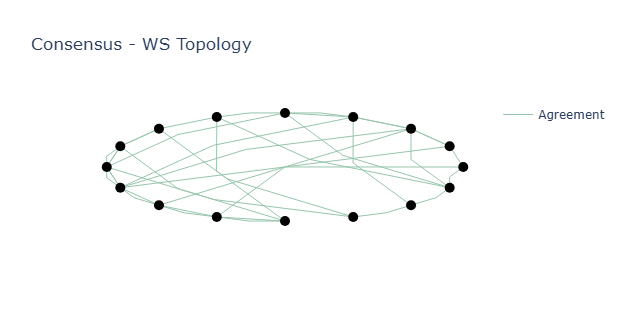
\includegraphics[trim=90 80 120 100,clip,width=0.19\textwidth]{figures/topology/consensus_results_20250917_231315_rounds7_gpt-4o-mini_nodes16.png}}
    \subfloat[SW ($n=50$)]{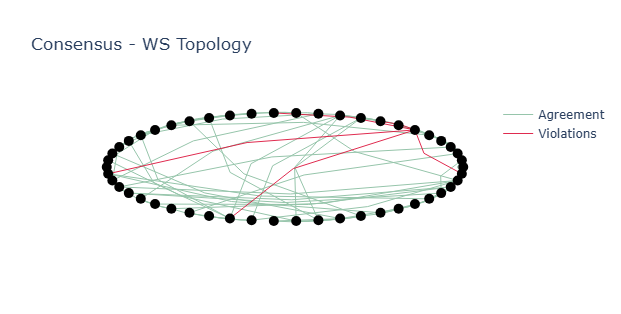
\includegraphics[trim=90 80 120 100,clip,width=0.22\textwidth]{figures/topology/consensus_results_20250919_171243_rounds11_gpt-4o-mini_nodes50.png}}
    \subfloat[SW ($n=100$)]{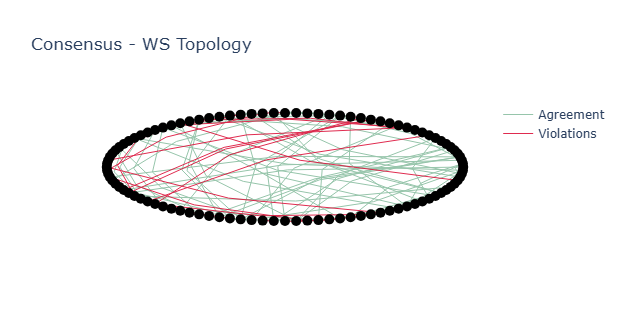
\includegraphics[trim=90 80 120 100,clip,width=0.26\textwidth]{figures/topology/consensus_results_20250919_143512_rounds15_gpt-4o-mini_nodes100.png}}



    
    \subfloat[SF ($n=4$)]{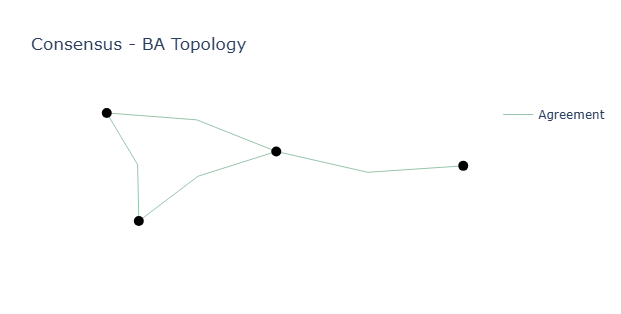
\includegraphics[trim=90 80 120 100,clip,width=0.12\textwidth]{figures/topology/consensus_results_20250917_231419_rounds5_gpt-4o-mini_nodes4.png}}
    \subfloat[SF ($n=8$)]{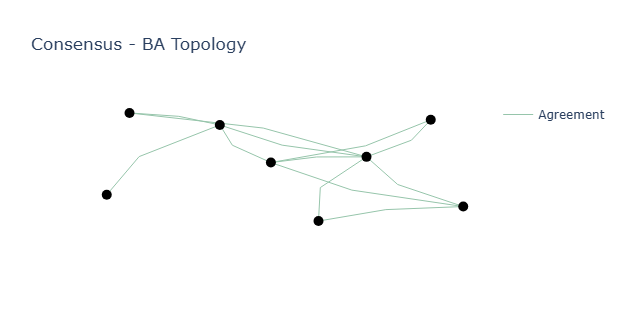
\includegraphics[trim=90 80 120 100,clip,width=0.16\textwidth]{figures/topology/consensus_results_20250917_231548_rounds7_gpt-4o-mini_nodes8.png}} 
    \subfloat[SF ($n=16$)]{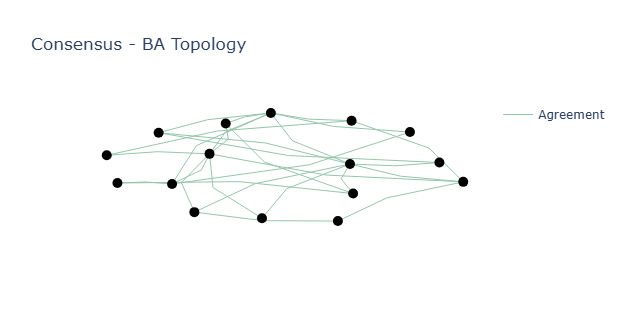
\includegraphics[trim=90 80 120 100,clip,width=0.19\textwidth]{figures/topology/consensus_results_20250917_231824_rounds9_gpt-4o-mini_nodes16.png}}
    \subfloat[SF ($n=50$)]{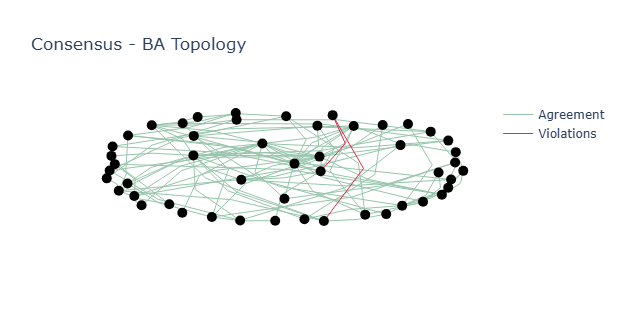
\includegraphics[trim=90 80 120 100,clip,width=0.22\textwidth]{figures/topology/consensus_results_20250919_173934_rounds11_gpt-4o-mini_nodes50.png}}
    \subfloat[SF ($n=100$)]{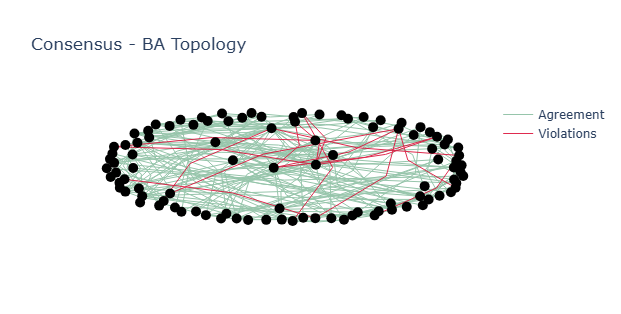
\includegraphics[trim=90 80 120 100,clip,width=0.26\textwidth]{figures/topology/consensus_results_20250919_180738_rounds11_gpt-4o-mini_nodes100.png}}

    
    \subfloat[DT ($n=4$)]{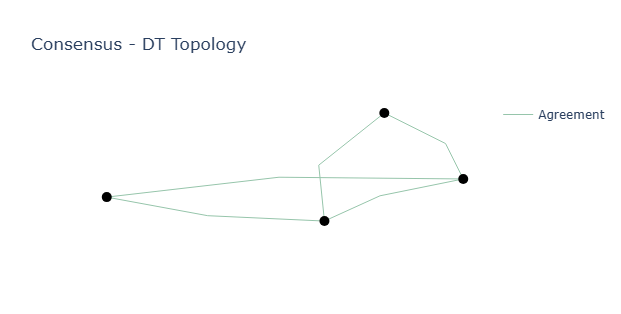
\includegraphics[trim=90 80 120 100,clip,width=0.12\textwidth]{figures/topology/consensus_results_20250917_231927_rounds5_gpt-4o-mini_nodes4.png}}
    \subfloat[DT ($n=8$)]{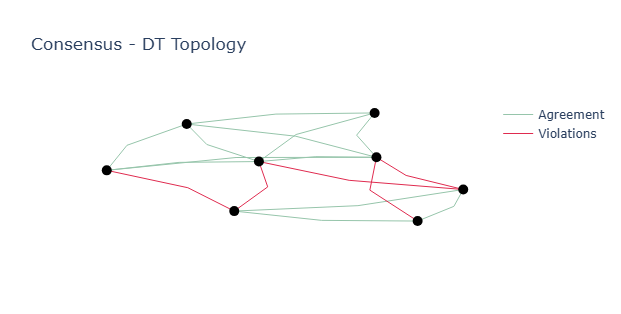
\includegraphics[trim=90 80 120 100,clip,width=0.16\textwidth]{figures/topology/consensus_results_20250917_232044_rounds5_gpt-4o-mini_nodes8.png}}
    \subfloat[DT ($n=16$)]{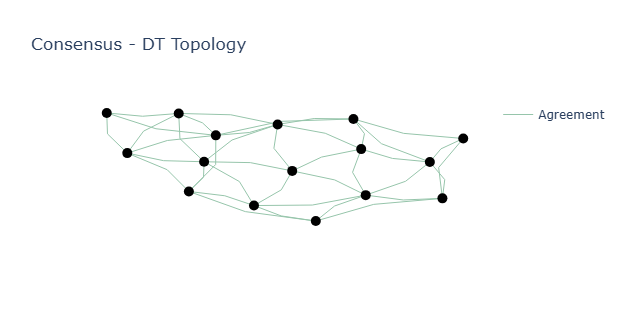
\includegraphics[trim=90 80 120 100,clip,width=0.19\textwidth]{figures/topology/consensus_results_20250917_232328_rounds9_gpt-4o-mini_nodes16.png}}
    \subfloat[DT ($n=50$)]{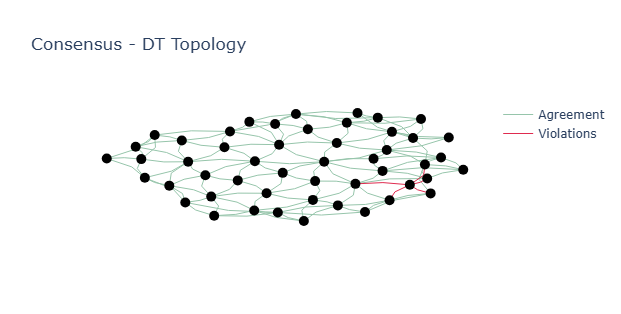
\includegraphics[trim=90 80 120 100,clip,width=0.22\textwidth]{figures/topology/consensus_results_20250919_182258_rounds13_gpt-4o-mini_nodes50.png}}
    \subfloat[DT ($n=100$)]{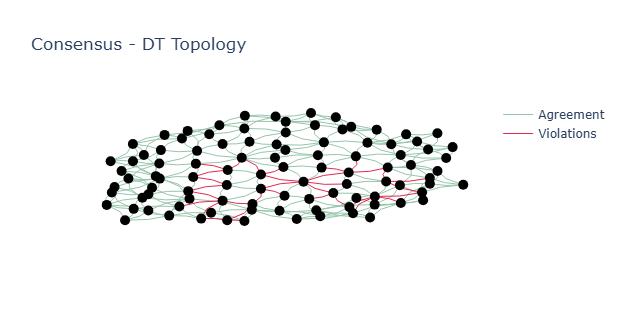
\includegraphics[trim=90 80 120 100,clip,width=0.26\textwidth]{figures/topology/consensus_results_20250919_185318_rounds19_gpt-4o-mini_nodes100.png}}


    
    


    \vspace{2mm}
    \subfloat[Seq ($n=4$)]{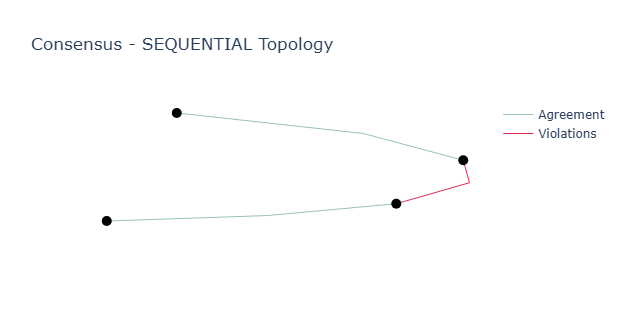
\includegraphics[trim=90 80 120 100,clip,width=0.12\textwidth]{figures/topology/consensus_results_20250924_141345_rounds7_gpt-4o-mini_nodes4.png}}
    \subfloat[Seq ($n=8$)]{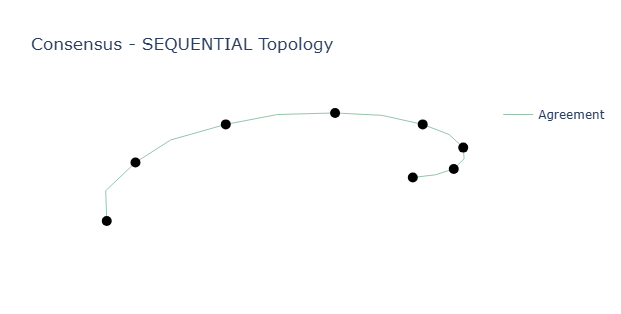
\includegraphics[trim=90 80 120 100,clip,width=0.16\textwidth]{figures/topology/consensus_results_20250924_141723_rounds15_gpt-4o-mini_nodes8.png}}
    \subfloat[Seq ($n=16$)]{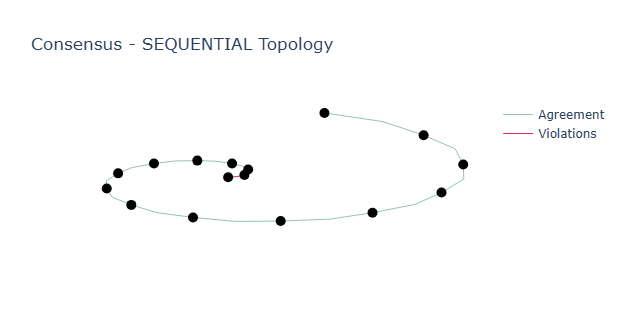
\includegraphics[trim=90 80 120 100,clip,width=0.19\textwidth]{figures/topology/consensus_results_20250924_142631_rounds31_gpt-4o-mini_nodes16.png}} 
    \subfloat{\rule{0.22\textwidth}{0pt}} % placeholder without number
    \subfloat{\rule{0.26\textwidth}{0pt}} % placeholder without number
    % \subfloat[Seq ($n=50$)]{
\includegraphics[trim=90 80 120 100,clip,width=0.22\textwidth]{figures/topology/consensus.png}} 
    % \subfloat[Seq ($n=100$)]{
\includegraphics[trim=90 80 120 100,clip,width=0.26\textwidth]{figures/topology/consensus.png}} 
    \\






    \subfloat[Hier ($n=4$)]{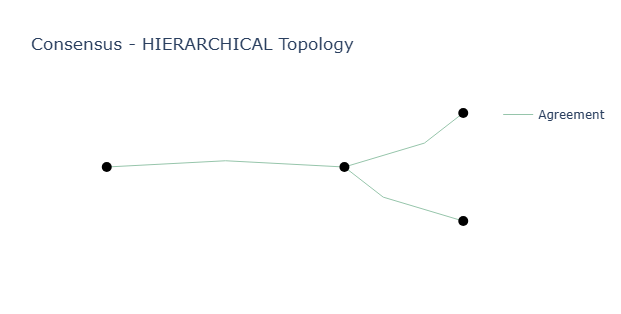
\includegraphics[trim=90 80 120 100,clip,width=0.12\textwidth]{figures/topology/consensus_results_20250924_145855_rounds5_gpt-4o-mini_nodes4.png}}
    \subfloat[Hier ($n=8$)]{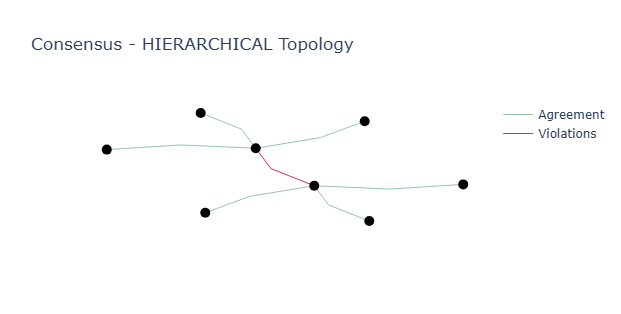
\includegraphics[trim=90 80 120 100,clip,width=0.16\textwidth]{figures/topology/consensus_results_20250924_150105_rounds7_gpt-4o-mini_nodes8.png}}
    \subfloat[Hier ($n=16$)]{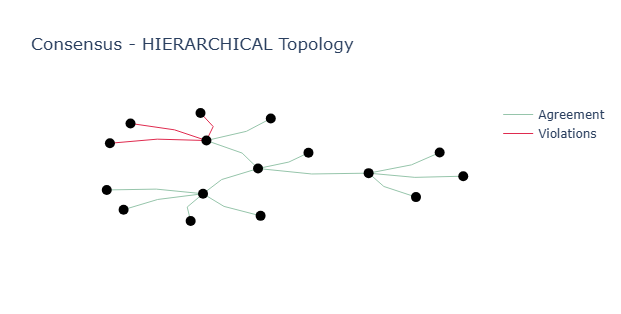
\includegraphics[trim=90 80 120 100,clip,width=0.19\textwidth]{figures/topology/consensus_results_20250924_150411_rounds9_gpt-4o-mini_nodes16}} 
    \subfloat[Hier ($n=50$)]{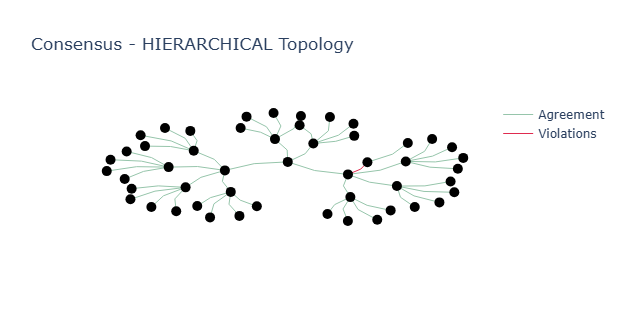
\includegraphics[trim=90 80 120 100,clip,width=0.22\textwidth]{figures/topology/consensus_results_20250926_115303_rounds13_gpt-4o-mini_nodes50.png}} 
    \subfloat[Hier ($n=100$)]{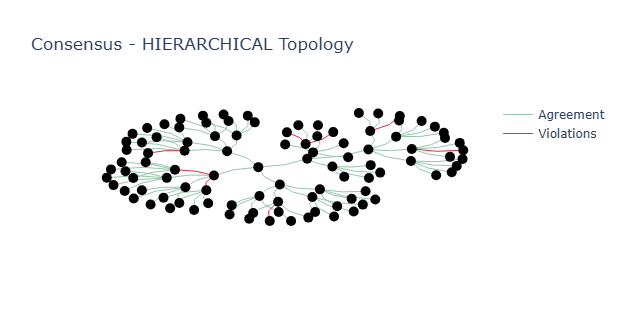
\includegraphics[trim=90 80 120 100,clip,width=0.26\textwidth]{figures/topology/consensus_results_20250926_120959_rounds15_gpt-4o-mini_nodes100.png}} \\
    


    \subfloat[All ($n=4$)]{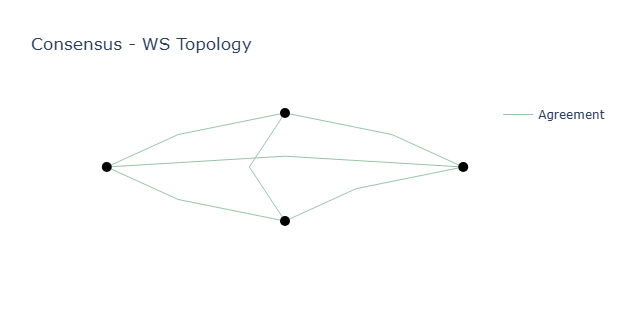
\includegraphics[trim=90 80 120 100,clip,width=0.12\textwidth]{figures/topology/consensus_results_20250917_232409_rounds3_gpt-4o-mini_nodes4.png}}
    \subfloat[All ($n=8$)]{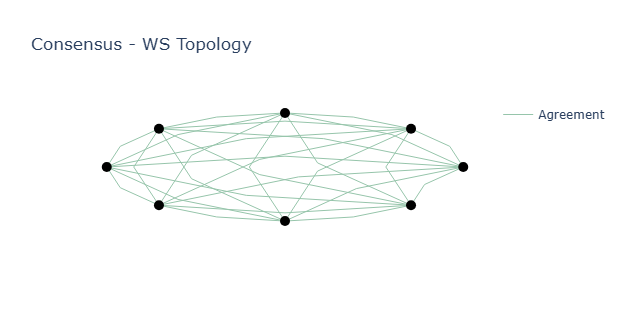
\includegraphics[trim=90 80 120 100,clip,width=0.16\textwidth]{figures/topology/consensus_results_20250917_232500_rounds3_gpt-4o-mini_nodes8.png}}
    \subfloat[All ($n=16$)]{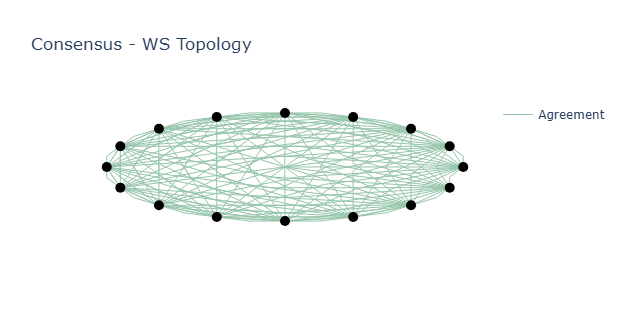
\includegraphics[trim=90 80 120 100,clip,width=0.19\textwidth]{figures/topology/consensus_results_20250917_232615_rounds3_gpt-4o-mini_nodes16.png}} 
    \subfloat[All ($n=50$)]{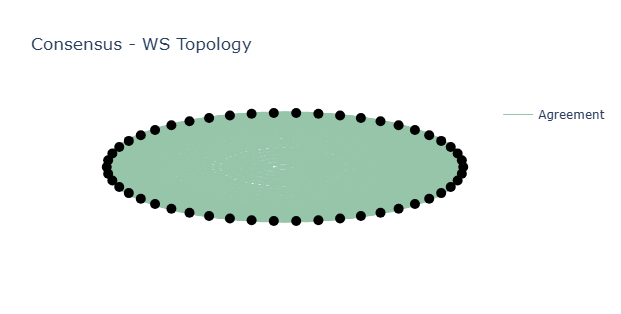
\includegraphics[trim=90 80 120 100,clip,width=0.22\textwidth]{figures/topology/consensus_results_20250919_165422_rounds3_gpt-4o-mini_nodes50.png}} 
    \subfloat[All ($n=100$)]{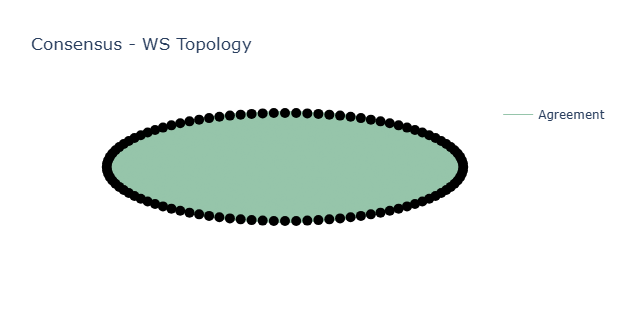
\includegraphics[trim=90 80 120 100,clip,width=0.26\textwidth]{figures/topology/consensus_results_20250919_102039_rounds3_gpt-4o-mini_nodes100.png}} \\

   


    
    \caption{Consensus experiment outcomes across different topologies and network sizes ($n=4$ to $100$).
Abbreviations denote topology classes: \textbf{SW} = Small-World, \textbf{SF} = Scale-Free, \textbf{DT} = Delaunay (geometric),
\textbf{Seq} = Sequential role-based pipeline, \textbf{Hier} = Hierarchical role-based orchestration, and
\textbf{All} = fully connected (all-to-all) communication.
Each subfigure visualizes the final agent states and their communication links.
\textbf{Green links} indicate agreement between two agents, while \textbf{red links} indicate disagreement or conflict.}
\label{fig:consensus-results}
\vspace{-4mm}
\end{figure*}




% \vspace{-1mm}
\vspace{-2mm}
\subsubsection{Communication, Coordination, and Scaling}
\label{sec:Coordination_section}

We evaluate how communication topology shapes coordination outcomes under constrained message passing using the AGENTSNET~\cite{coordinationcollaborativereasoning} benchmark. All experiments fix the model backend, task definitions, prompts, execution protocol, and round budgets through the unified MAFBench infrastructure, while varying only the interaction structure. We compare representative topology classes including graph-based communication (small-world~\cite{watts1998collective}, scale-free~\cite{scale_free}, and Delaunay~\cite{delaunay}), role-based pipelines (sequential and hierarchical), and centralized broadcast-style interaction implemented via star-shaped graphs. Network size varies over \(n \in \{4, 8, 16, 50, 100\}\). We report task success, rounds to convergence, token usage, and runtime (Table~\ref{tab:scalability-results}). For bounded tasks, a minimum of eight interaction rounds is enforced. For global agreement tasks (\emph{LeaderElection} and \emph{Consensus}), success is binary rather than graded. Detailed configurations, success definitions for all tasks, and metric formulations are provided in Appendix~\ref{appendix:extended}. The maximum interaction rounds follow \(T = 2D + 1\), where \(D\) is the graph diameter, ensuring sufficient information propagation.\footnote{The graph diameter \(D\) is the maximum shortest-path distance between any pair of nodes in the communication graph.}


Results show that coordination performance is governed primarily by the match between task structure and communication geometry. Increasing communication volume, rounds, or token budgets alone does not consistently improve outcomes. For local coordination tasks such as \emph{Coloring} and \emph{Matching}, topologies that preserve neighborhood structure achieve higher success. Scale-free graphs reach near-perfect success at large scale, for example achieving \(0.97\) on Coloring at \(n=100\). They also converge in substantially fewer rounds and lower token cost than small-world graphs (\(5{,}699\text{k}\) vs.\ \(10{,}431\text{k}\) tokens). Small-world graphs remain effective but incur growing coordination overhead as network size increases. Delaunay topologies exhibit higher instability and collapse entirely for Matching at large scale. Centralized broadcast interaction converges rapidly but achieves only moderate success on \emph{Matching}, showing that fast information mixing alone does not ensure correct coordination.



For global constraint satisfaction and agreement tasks, topology dependence becomes more pronounced. In \emph{VertexCover}, small-world graphs perform better at small scale, while scale-free graphs dominate at large scale in both success and efficiency, achieving higher success with fewer rounds and lower token cost. For \emph{LeaderElection}, both small-world and scale-free structures fail across all sizes, while Delaunay graphs succeed only at moderate and large scale at high coordination cost due to long confirmation paths. Role-based hierarchies and centralized interaction succeed only at very small scale and degrade rapidly. For strict global agreement in \emph{Consensus}, the fully connected topology is the only structure that succeeds consistently, converging in three rounds independent of network size, while all graph-based topologies fail despite substantially higher runtime and token expenditure. Figure~\ref{fig:consensus-results} illustrates representative consensus dynamics under different topologies, highlighting fragmentation and delayed mixing in graph-based structures versus immediate convergence under broadcast. Notably, disagreement clusters persist as network size grows in sparse topologies. Additional visualizations for all coordination tasks and topologies are provided in Appendix~\ref{appendix:extended}.

These results demonstrate that coordination scalability is an architectural property of communication structure rather than a consequence of increased interaction budgets or LLM capability. Performance is driven by how frameworks impose information flow between agents. Local coordination benefits from sparse topologies that preserve neighborhood structure. Global agreement requires dense connectivity to avoid fragmentation. No single topology achieves robust performance across all coordination tasks. Effective multi-agent system design therefore requires selecting communication architectures that match task-specific information flow patterns, rather than increasing rounds, tokens, or model capacity to compensate for misaligned interaction structure.



\captionsetup[subfigure]{labelformat=empty}

\setlength{\abovecaptionskip}{2pt}
\setlength{\belowcaptionskip}{0pt}

\begin{figure*}[t]
\vspace{-2mm}
    \centering
    % --- Small sizes ---
    \subfloat[SW ($n=4$)]{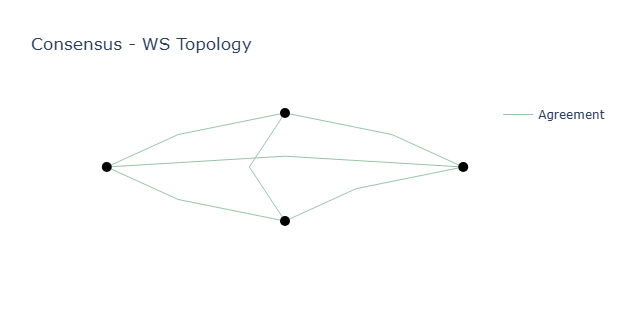
\includegraphics[trim=90 80 120 100,clip,width=0.12\textwidth]{figures/topology/consensus_results_20250917_230934_rounds3_gpt-4o-mini_nodes4.png}}
    \subfloat[SW ($n=8$)]{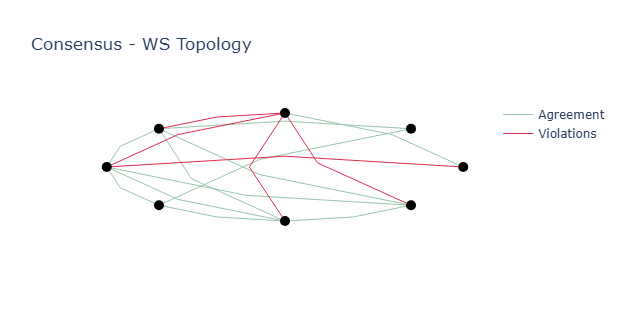
\includegraphics[trim=90 80 120 100,clip,width=0.16\textwidth]{figures/topology/consensus_results_20250917_231133_rounds7_gpt-4o-mini_nodes8.png}}
    \subfloat[SW ($n=16$)]{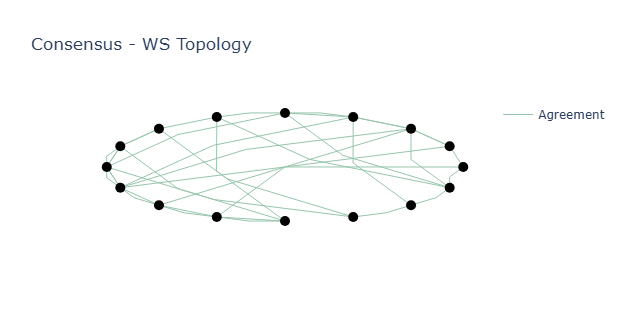
\includegraphics[trim=90 80 120 100,clip,width=0.19\textwidth]{figures/topology/consensus_results_20250917_231315_rounds7_gpt-4o-mini_nodes16.png}}
    \subfloat[SW ($n=50$)]{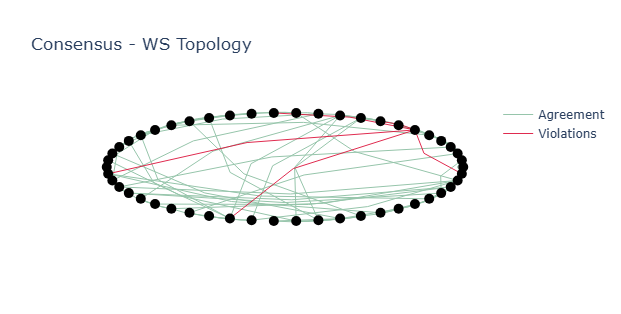
\includegraphics[trim=90 80 120 100,clip,width=0.22\textwidth]{figures/topology/consensus_results_20250919_171243_rounds11_gpt-4o-mini_nodes50.png}}
    \subfloat[SW ($n=100$)]{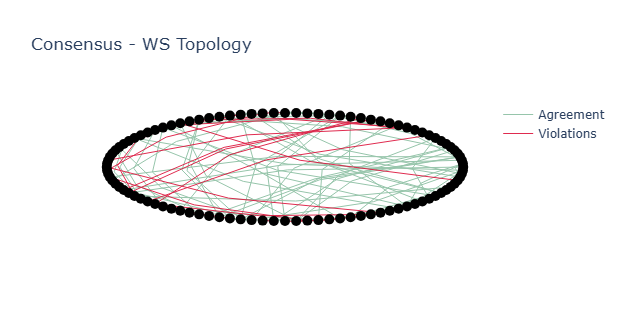
\includegraphics[trim=90 80 120 100,clip,width=0.26\textwidth]{figures/topology/consensus_results_20250919_143512_rounds15_gpt-4o-mini_nodes100.png}}



    
    \subfloat[SF ($n=4$)]{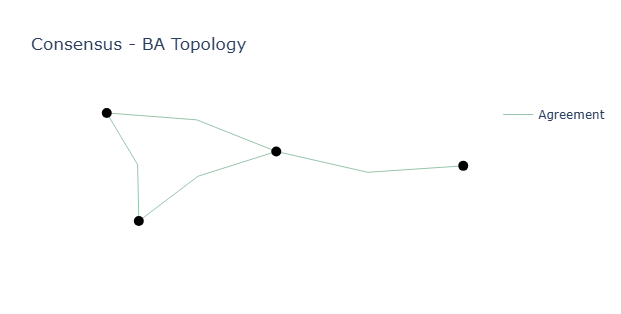
\includegraphics[trim=90 80 120 100,clip,width=0.12\textwidth]{figures/topology/consensus_results_20250917_231419_rounds5_gpt-4o-mini_nodes4.png}}
    \subfloat[SF ($n=8$)]{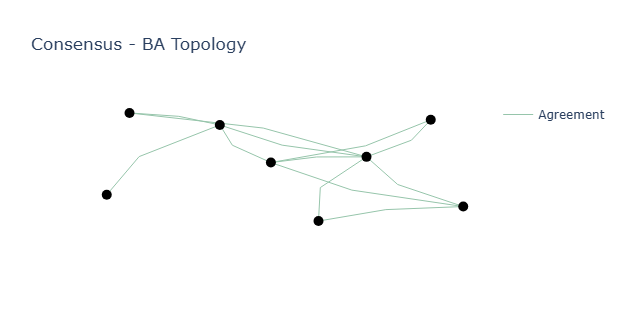
\includegraphics[trim=90 80 120 100,clip,width=0.16\textwidth]{figures/topology/consensus_results_20250917_231548_rounds7_gpt-4o-mini_nodes8.png}} 
    \subfloat[SF ($n=16$)]{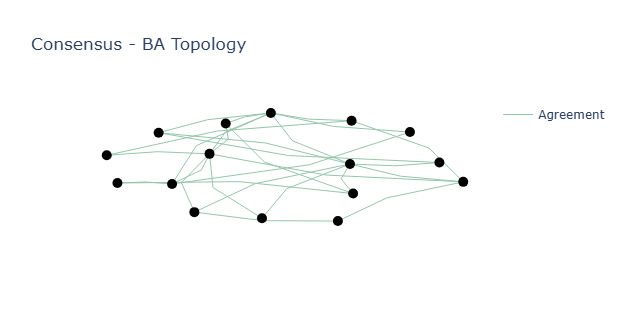
\includegraphics[trim=90 80 120 100,clip,width=0.19\textwidth]{figures/topology/consensus_results_20250917_231824_rounds9_gpt-4o-mini_nodes16.png}}
    \subfloat[SF ($n=50$)]{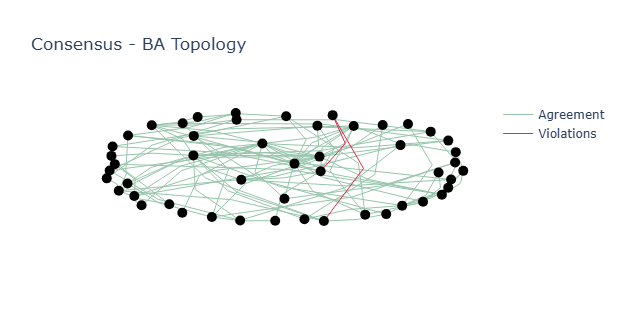
\includegraphics[trim=90 80 120 100,clip,width=0.22\textwidth]{figures/topology/consensus_results_20250919_173934_rounds11_gpt-4o-mini_nodes50.png}}
    \subfloat[SF ($n=100$)]{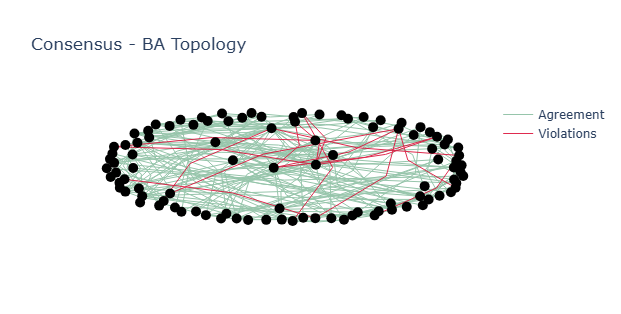
\includegraphics[trim=90 80 120 100,clip,width=0.26\textwidth]{figures/topology/consensus_results_20250919_180738_rounds11_gpt-4o-mini_nodes100.png}}

    
    \subfloat[DT ($n=4$)]{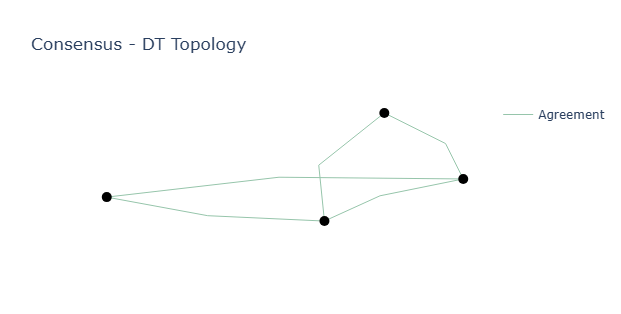
\includegraphics[trim=90 80 120 100,clip,width=0.12\textwidth]{figures/topology/consensus_results_20250917_231927_rounds5_gpt-4o-mini_nodes4.png}}
    \subfloat[DT ($n=8$)]{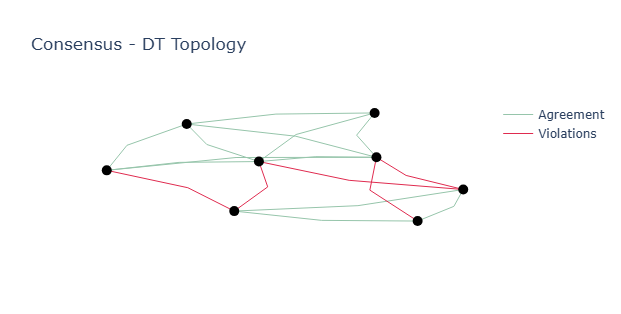
\includegraphics[trim=90 80 120 100,clip,width=0.16\textwidth]{figures/topology/consensus_results_20250917_232044_rounds5_gpt-4o-mini_nodes8.png}}
    \subfloat[DT ($n=16$)]{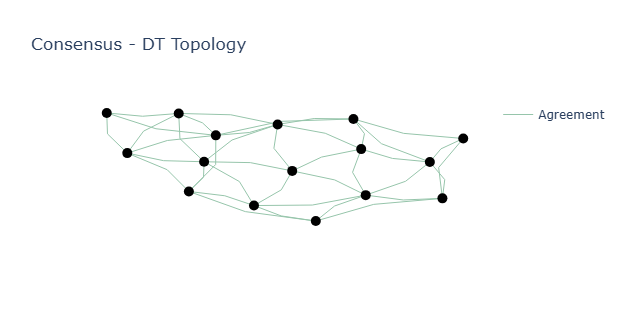
\includegraphics[trim=90 80 120 100,clip,width=0.19\textwidth]{figures/topology/consensus_results_20250917_232328_rounds9_gpt-4o-mini_nodes16.png}}
    \subfloat[DT ($n=50$)]{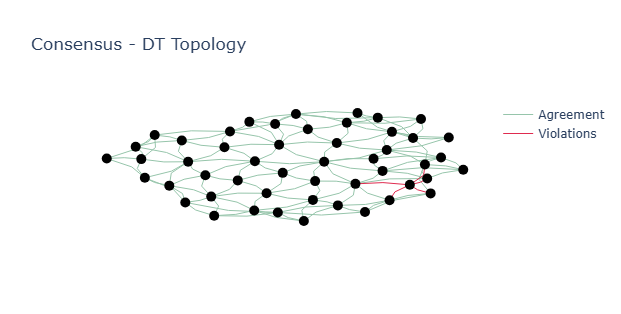
\includegraphics[trim=90 80 120 100,clip,width=0.22\textwidth]{figures/topology/consensus_results_20250919_182258_rounds13_gpt-4o-mini_nodes50.png}}
    \subfloat[DT ($n=100$)]{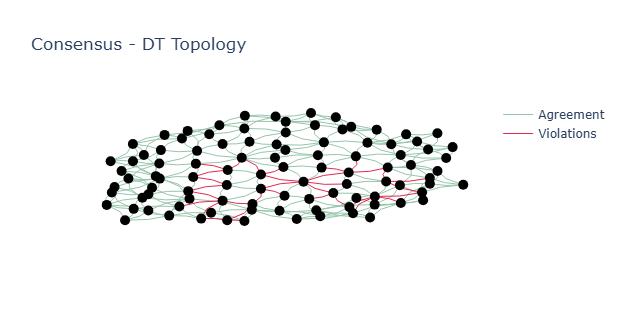
\includegraphics[trim=90 80 120 100,clip,width=0.26\textwidth]{figures/topology/consensus_results_20250919_185318_rounds19_gpt-4o-mini_nodes100.png}}


    
    


    \vspace{2mm}
    \subfloat[Seq ($n=4$)]{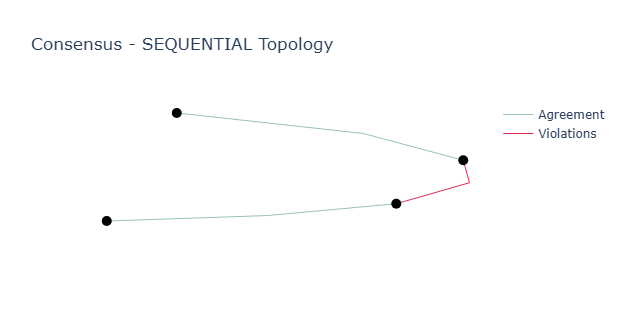
\includegraphics[trim=90 80 120 100,clip,width=0.12\textwidth]{figures/topology/consensus_results_20250924_141345_rounds7_gpt-4o-mini_nodes4.png}}
    \subfloat[Seq ($n=8$)]{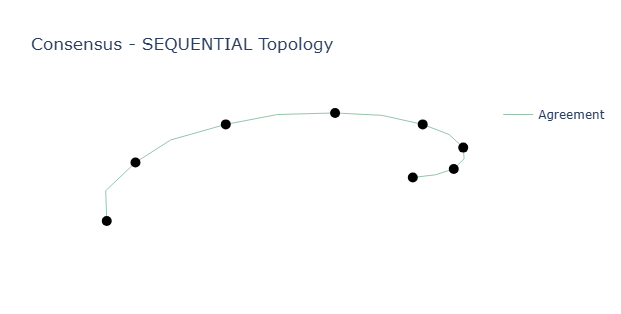
\includegraphics[trim=90 80 120 100,clip,width=0.16\textwidth]{figures/topology/consensus_results_20250924_141723_rounds15_gpt-4o-mini_nodes8.png}}
    \subfloat[Seq ($n=16$)]{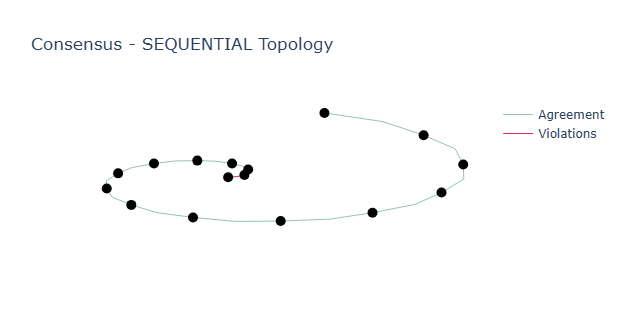
\includegraphics[trim=90 80 120 100,clip,width=0.19\textwidth]{figures/topology/consensus_results_20250924_142631_rounds31_gpt-4o-mini_nodes16.png}} 
    \subfloat{\rule{0.22\textwidth}{0pt}} % placeholder without number
    \subfloat{\rule{0.26\textwidth}{0pt}} % placeholder without number
    % \subfloat[Seq ($n=50$)]{
\includegraphics[trim=90 80 120 100,clip,width=0.22\textwidth]{figures/topology/consensus.png}} 
    % \subfloat[Seq ($n=100$)]{
\includegraphics[trim=90 80 120 100,clip,width=0.26\textwidth]{figures/topology/consensus.png}} 
    \\






    \subfloat[Hier ($n=4$)]{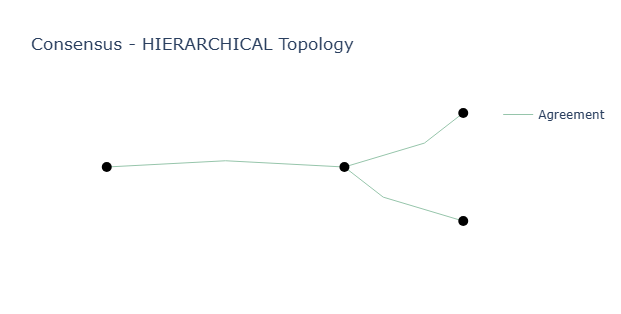
\includegraphics[trim=90 80 120 100,clip,width=0.12\textwidth]{figures/topology/consensus_results_20250924_145855_rounds5_gpt-4o-mini_nodes4.png}}
    \subfloat[Hier ($n=8$)]{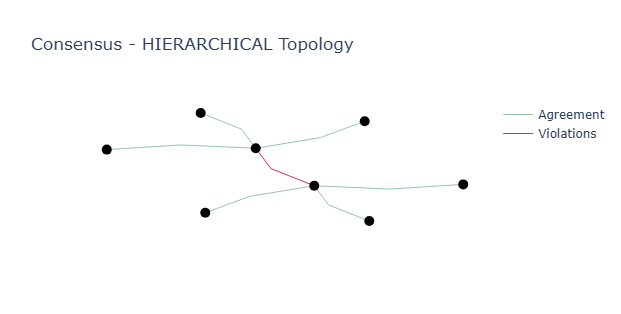
\includegraphics[trim=90 80 120 100,clip,width=0.16\textwidth]{figures/topology/consensus_results_20250924_150105_rounds7_gpt-4o-mini_nodes8.png}}
    \subfloat[Hier ($n=16$)]{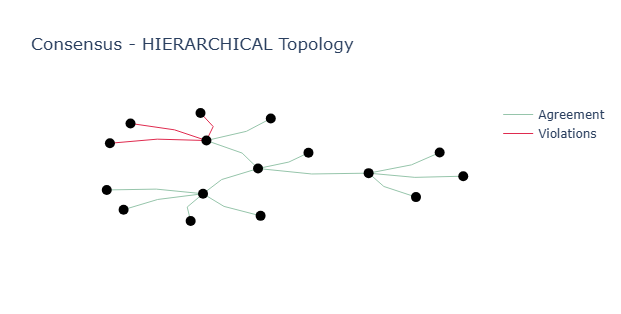
\includegraphics[trim=90 80 120 100,clip,width=0.19\textwidth]{figures/topology/consensus_results_20250924_150411_rounds9_gpt-4o-mini_nodes16}} 
    \subfloat[Hier ($n=50$)]{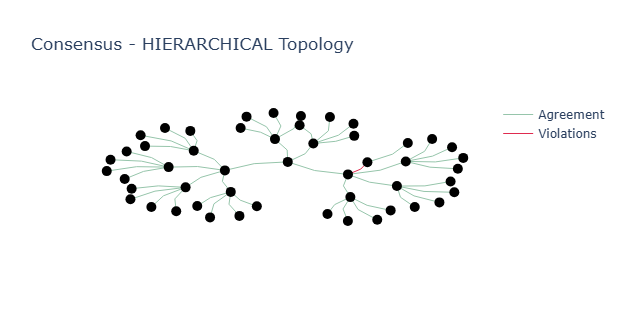
\includegraphics[trim=90 80 120 100,clip,width=0.22\textwidth]{figures/topology/consensus_results_20250926_115303_rounds13_gpt-4o-mini_nodes50.png}} 
    \subfloat[Hier ($n=100$)]{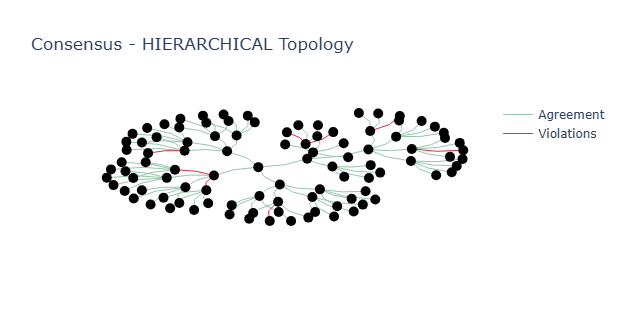
\includegraphics[trim=90 80 120 100,clip,width=0.26\textwidth]{figures/topology/consensus_results_20250926_120959_rounds15_gpt-4o-mini_nodes100.png}} \\
    


    \subfloat[All ($n=4$)]{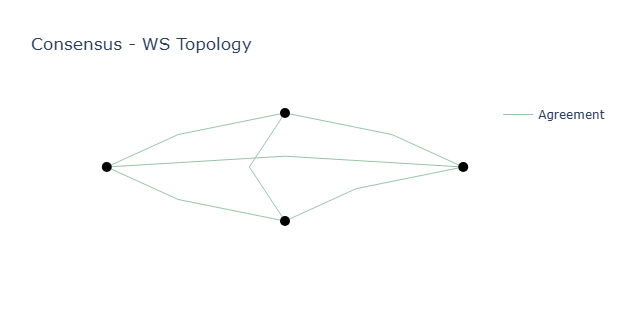
\includegraphics[trim=90 80 120 100,clip,width=0.12\textwidth]{figures/topology/consensus_results_20250917_232409_rounds3_gpt-4o-mini_nodes4.png}}
    \subfloat[All ($n=8$)]{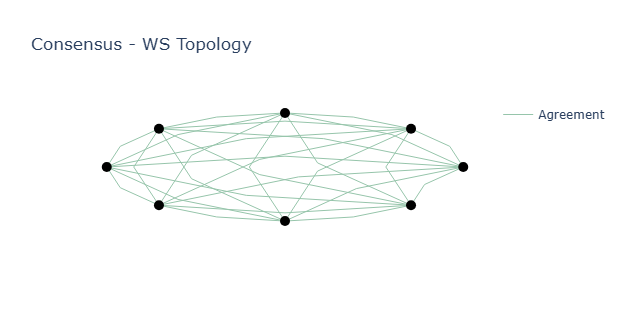
\includegraphics[trim=90 80 120 100,clip,width=0.16\textwidth]{figures/topology/consensus_results_20250917_232500_rounds3_gpt-4o-mini_nodes8.png}}
    \subfloat[All ($n=16$)]{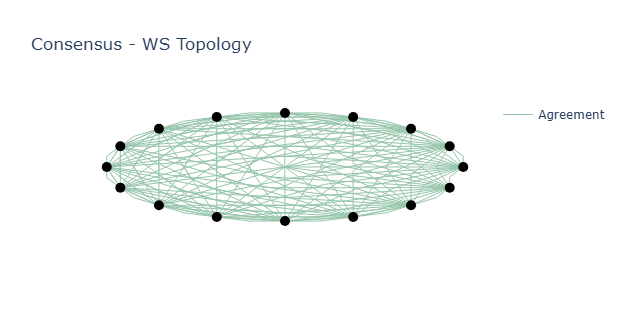
\includegraphics[trim=90 80 120 100,clip,width=0.19\textwidth]{figures/topology/consensus_results_20250917_232615_rounds3_gpt-4o-mini_nodes16.png}} 
    \subfloat[All ($n=50$)]{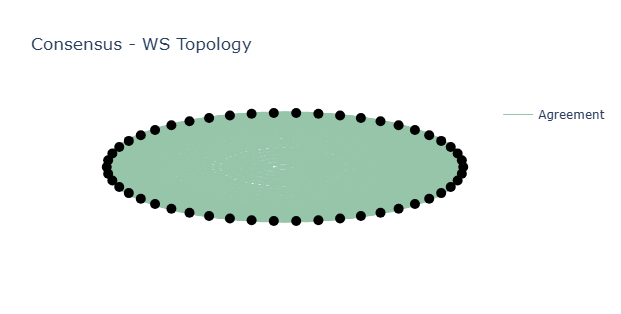
\includegraphics[trim=90 80 120 100,clip,width=0.22\textwidth]{figures/topology/consensus_results_20250919_165422_rounds3_gpt-4o-mini_nodes50.png}} 
    \subfloat[All ($n=100$)]{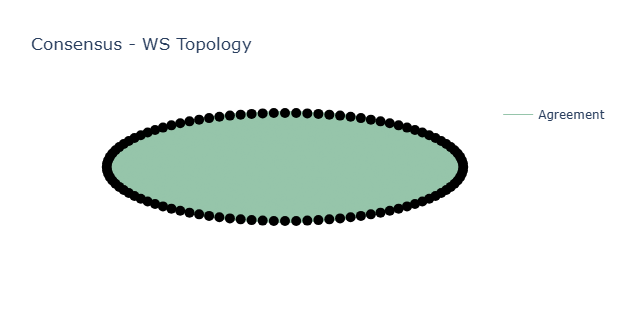
\includegraphics[trim=90 80 120 100,clip,width=0.26\textwidth]{figures/topology/consensus_results_20250919_102039_rounds3_gpt-4o-mini_nodes100.png}} \\

   


    
    \caption{Consensus experiment outcomes across different topologies and network sizes ($n=4$ to $100$).
Abbreviations denote topology classes: \textbf{SW} = Small-World, \textbf{SF} = Scale-Free, \textbf{DT} = Delaunay (geometric),
\textbf{Seq} = Sequential role-based pipeline, \textbf{Hier} = Hierarchical role-based orchestration, and
\textbf{All} = fully connected (all-to-all) communication.
Each subfigure visualizes the final agent states and their communication links.
\textbf{Green links} indicate agreement between two agents, while \textbf{red links} indicate disagreement or conflict.}
\label{fig:consensus-results}
\vspace{-4mm}
\end{figure*}
